\documentclass[../main.tex]{subfiles}
\graphicspath{
    {"../img/"}
    {"img/"}
}
\begin{document}

\begin{align*}
f(x_0+h) = f(x_0) + &\sum_{i=1}^n \frac{\partial f}{\partial x^i} (x_0) h^i + \frac{1}{2!}\sum_{\substack{i=1\\ j=1}}^n \frac{\partial^2 f}{\partial x^i \partial x^j} (x_0) h^i h^j  + \dots + \frac{1}{p!}  \\
&\sum_{\substack{i_1 = 1\\ \vdots \\ i_p = 1}}^n \frac{\partial^p f}{\partial x^{i_1} \dots \partial x^{i_p+1}} (x_0) h^{i_1} \dots h^{i_p} + R_{p+1} (x_0, h)
\end{align*}
$$\text{gdzie } R_{p+1} (h) = \frac{1}{(p+1)!} \sum_{\substack{i_1 = 1\\ \dots \\i_{p+1} = 1}}^n \frac{\partial^{p+1} f}{\partial x^{i_1} \dots \partial x^{i_p+1}} \underset{\substack{0<\theta<1\\ \text{ wersja } \mathbb{R}^n \text{ dla }\\"x_0 < c < x_0 +h"}}{(x_0+\theta h)} h^{i_1} \dots h^{i_{p+1}}$$

\begin{obserwacja}
$\lim\limits_{h \to 0}\frac{R_{p+1} (x_0,h)}{||h||^p} \to 0$
\end{obserwacja}

\begin{przyklad}

\end{przyklad}
$f: \mathbb{R}^2 \to \mathbb{R}, \quad f(x,y) = x^2y^3, f'(x,y) = \Big [ 2xy^3, 3x^2y^2 \Big ]$.

Jeżeli $h = \left [ \begin{matrix}
h_1\\
h_2\\
 \end{matrix}\right ]$, to wtedy
\begin{align*}
\sum_{\substack{i=1 \\ j=1}}^2 \frac{\partial^2 f}{\partial x^i \partial x^j} h^i h^j
&=\frac{\partial^2 f}{\partial x^1 \partial x^1} h^1 h^1 + \frac{\partial^2 f}{\partial x^1 \partial x^2} h^1 h^2 + \frac{\partial^2 f}{\partial x^2 \partial x^1} h^2 h^1 + \frac{\partial^2 f}{\partial x^2 \partial x^2} h^2 h^2 =\\
&= \Big [ h_1, h_1 \Big ] \left [ \begin{matrix}
\frac{\partial^2 f}{\partial x_1^2}  &\frac{\partial^2 f}{\partial x_1 \partial x_2} \\
\frac{\partial^2 f}{\partial x_2 \partial x_1}  &\frac{\partial^2 f}{\partial x_2^2}  \end{matrix}\right ] \left [ \begin{matrix}
h_1\\
h_2 \end{matrix}\right ]
\end{align*}

To czy ta macierz jest uśmiechnięta etc. (dodatnio/ujemnie określona) na algebrze.

\begin{large}
    Minima i maksima
\end{large}


\begin{large}
Przypomnienie
\end{large}
Niech $f: \mathcal{O}\to \mathbb{R}, \mathcal{O}\subset \mathbb{R}^n, \mathcal{O}$ - otwarty, $x_0 \in \mathcal{O}$\\
Mówimy, że $f$ ma w $x_0$ minimum lokalne, jeżeli:
$$\underset{\eta > 0}{\exists} \quad
\underset{\substack{
x\in K(x_0,\eta)\\
K(x_0,\eta) \subset \mathcal{O}\\
x \neq x_0
}}{\forall} \quad f(x) > f(x_0), \{f(x) < f(x_0)\} \leftarrow \text { maksimum}$$

Albo inaczej:
$$\underset{\eta > 0}{\exists} \quad\underset{h}{\forall}\quad ||h|| < \eta, \quad x_0+h \in \mathcal{O}, h \neq 0\text{, to wtedy } f(x_0+h)>f(x_0)$$

\begin{figure}[h]
    \centering
    \includegraphics[width=0.5\textwidth]{fig_12}
    \caption{istnieje otoczenie, dla którego  $f(x)>f(x_0)$ (nie musi być styczne!)}
\end{figure}

\begin{figure}[h]
    \centering
    \includegraphics[width=0.8\textwidth]{fig_13}
    \caption{}
    \label{fig:}
\end{figure}

\begin{stw}
jeżeli $f: \mathcal{O} \rightarrow \mathbb{R}, \mathcal{O}$ - otwarty, $x_0 \in \mathcal{O}, f$ - posiada w $x_0$ minimum lub maksimum lokalne, to $$\frac{\partial f}{\partial x^i} (x_0) = 0, i = 1,\dots,n$$
(działa tylko w prawo, bo możliwe punkty przegięcia ((siodła)) )
\end{stw}

\vspace{1cm}
\begin{dowod}

\end{dowod}
Niech $g_h (t) = f(x_0+th) \text{ i } g: [0,\epsilon [ \to \mathbb{R}$.\\
Zauważmy, że jeżeli $f$ ma minimum lub maksimum w $x_0$, to znaczy, że $g_h (t)$ ma minimum lub maksimum w $t = 0$, czyli $\left . \frac{\partial}{\partial t} g_h(t) \right |_{t=0}$

Czyli:
\begin{align*}
    &x_0 = \big ( x_0^1, x_0^2, \dots, x_0^n)\\
    &h = \big ( h^1, h^2, \dots, h^n)\\
\end{align*}

\begin{align*}
&\left . \frac{d}{dt} g_h (t) \right |_{t=0} = \left .\frac{d}{dt} f(x_0^1 + th^1, \dots, x_0^n + th^n) \right |_{t=0} = \\
& \frac{\partial f}{\partial x^1} (x_0 + th^1) h^1 + \frac{\partial f}{\partial x^2} (x_0 + th^2) h^2 + \dots + \left .\frac{\partial f}{\partial x^n} (x_0 + th^n) \right |_{t=0}=\\
&=\sum_{i=1}^n \frac{\partial f}{\partial x^i} (x_0) h^i = 0 \quad |\underset{h}{\forall}: ||h|| < \eta \text{, to znaczy: }\frac{\partial f}{\partial x^i} (x_0) = 0_{i = 1,\dots,n} \Box
\end{align*}

\begin{tw}
Niech $f: \mathcal{O} \to \mathbb{R}, \quad\mathcal{O}\subset\mathbb{R}^n, \quad x_0\in\mathcal{O}, \quad \mathcal{O} \text{ - otwarty, a } f \text{ - klasy } C^{2p} (\mathcal{O})$ oraz $f'(x_0) = 0, f''(x_0) = 0,\dots,f^{(2p-1)} (x_0) = 0$
i $$\underset{c > 0}{\exists} \quad\underset{\eta > 0}{\exists} \quad\underset{h\in K(x_0,\eta)}{\forall}: \quad \sum_{\substack{i_1 = 1\\ \vdots \\ i_{2p} = 1}}^n \frac{\partial^{(2p)} f}{\partial x^{i_1} \dots \partial x^{i_{2p}}} (x_0) h^{i_1} \dots h^{i_{2p}} \geq c ||h||^{2p} (\leq c||h||^{2p})$$
to $f$ ma w $x_0$ minimum (maksimum) lokalne.
\end{tw}

\vspace{1cm}
\begin{dowod}
    (dla minimum)

(wersja uproszczona dla $f$ klasy $C^{2p+1}(\mathcal{O}))$
\end{dowod}

Jeżeli $f$ spełnia założenie z twierdzenia, to wtedy $$f(x_0+h)-f(x_0) = \frac{1}{(2p)!} (\Delta)\sum_{\substack{i_1 = 1\\ \vdots \\ i_{2p} = 1}}^{2p} \frac{\partial^{(2p)} f(x_0)}{\partial x^{i_1} \dots x^{i_{(2p)}}} h^{i_1} \dots h^{i_{(2p)}} + r_{2p + 1} (x_0 + h)$$

Wiemy też , że $\underset{c > 0}{\exists}\quad \underset{\eta > 0}{\exists} \underset{\substack{\text{Chodzi o to, żeby reszta}\\ \text{ nie mogła tego przekroczyć}}}{\quad(\Delta) \geq c ||h||^{2p}}$

Chcemy pokazać, że $\underset{\eta}{\exists} \quad \underset{||h||<\eta}{\forall} \Big | r_{2p+1} (x,h) \Big | \leq \underset{\substack{\text{albo 7,}\\ \text{albo 2019}}}{\frac{c}{2} ||h||^{2p}}$

Czyli chcemy zbadać wielkość:
$$ \frac{1}{(2p+1)!} \sum_{\substack{i_1 = 1 \\ \vdots \\ i_{2p+1} = 1}}^n \underset{0 < \theta < 1}{\frac{\partial^{(2p+1)} f (x_0 + \theta h)}{\partial x^{i_1} \dots \partial x^{i_{(2p+1)}}}} h^{i_1} \dots h^{i_{(2p+1)}} = \text{ /*tu potrzebne założenie, że } f \text { - klasy } C^{2p+1} (\mathcal{O})\text{*/} = r_{2p+1} (x,h)$$

Zauważmy, że $\lim\limits_{h \to 0} \frac{r_{2p+1}(x_0+h)}{||h||^{2p}} \to 0$, ale zatem
$$\underset{M>0}{\forall}\quad \underbrace{\underset{N}{\exists},\underset{n>N}{\forall}}_{\substack{\text{bez sensu!}\\
\underset{\eta}{\exists},\underset{||h|| < \eta}{\forall}}} \frac{r_{2p+1}(x_0+h)}{||h||^{2p}} < M$$

$$\text{czyli: } \Bigg | \frac{r_{2p+1} (x_0,h)}{||h||^{2p}} \Bigg | < M$$

$$\underset{M}{\forall}\quad \underset{\eta}{\exists} \underset{||h|| < \eta}{\forall}\quad \Big | r_{2p+1} (x_0,h) \Big | < M \big | \big |h \big | \big |^{2p}$$
Kładziemy $M = \frac{c}{2}$ i mamy
$$\underset{\eta}{\exists},\underset{||h||<\eta}{\forall}\quad f(x_0+h)-f(x_0) \geq \frac{c}{2} ||h||^{2p} \quad \Box $$

\begin{large}
    Uwaga:
\end{large}
Dlaczego warunek $( | \big | | ) > c ||h||^{2p}$, a nie po prostu $( ) > 0$?

\begin{przyklad}

\end{przyklad}
$f(x,y) = x^2 + y^4,\quad \frac{\partial f}{\partial x} = 2x,\quad \frac{\partial f}{\partial y} = 4y^3$.\\
$f'() = 0 \iff (x,y) = (0,0)$\\
Badamy: $f(0+h) - f(0) = \big [ h_1, h_2 \big ] \left [ \begin{matrix}
2 &0\\
0 &2y^2\\
\end{matrix}\right ]
\left [ \begin{matrix}
h_1\\
h_2\\\end{matrix}\right ]
= \big [ h_1, h_2 \big ] \left [ \begin{matrix}
2 &0\\
0 &0\\ \end{matrix}\right ]
\left [ \begin{matrix} h_1\\
h_2\end{matrix}\right ] = 2h_1^2$

Czyli $f(0+h) - f(0) ~ 2h_1^2$ - minimum? maksimum? - zależy w którą stronę.\\
$h = \left [ \begin{matrix}
h_1\\
0\\
\end{matrix}\right ] $ - minimum\\
$h = \left [ \begin{matrix}
0\\
h_2\\
\end{matrix}\right ] $ - równo.\\
Coś takiego - siodło.

Widzimy zatem, że nie jest spełniony warunek $\underset{c}{\exists}\big [ h_1, h_2 \big ] \left [ \begin{matrix}
2 &0\\
0 &0\\
\end{matrix}\right ]
\left [ \begin{matrix}
h_1\\
h_2\\
    \end{matrix}\right ] \geq c \big | \big | h \big | \big | ^2$, bo dla $h = \left [ \begin{matrix}
0\\
h_2\\
    \end{matrix}\right ] \quad 0 \not\geq c \Bigg | \Bigg | \left [ \begin{matrix}
0\\
h_2\\
\end{matrix}\right ] \Bigg |\Bigg |$

\begin{large}
    Kilka fajnych zastosowań
\end{large}
$$\frac{mv^2}{2} =
\left [ \begin{matrix}
 &v &\\ \end{matrix}\right ]
\left [ \begin{matrix}
    \frac{m}{2}\\
&\frac{m}{2}\\
   & & \ddots\\
    \end{matrix}\right ]  \left [ \begin{matrix}
\\
v\\
 \\\end{matrix}\right ]$$
 $$\frac{I \omega^2}{2} =
 \left [ \begin{matrix}
 &\omega &
 \\ \end{matrix}\right ]
 \left [ \begin{matrix}
 - &- &-\\
 - &- &-\\
 - &- &-\\
     \end{matrix}\right ] \left [ \begin{matrix}
 \\
 \omega\\
 \\
 \end{matrix}\right ] $$

\end{document}
